非常に多くの分野で活用されるようになったDeepLearning技術だが,モデルの性能向上に伴い計算に必要な資源も増加している.

\begin{table}[H]
	\caption{FLOPs vs Weights}
	\label{table:flops_vs_weights}
	\centering
	\begin{tabular}{lll}
		\hline
		Model Name & FLOPs & Weights \\ 
		\hline \hline 
		Xception & 8357403496 & 22801424 \\ 
		VGG16 & 15470264320 & 138357544 \\ 
		VGG19 & 19632062464 & 143667240 \\ 
		ResNet50 & 3857973248 & 25530472 \\ 
		ResNet101 & 7570194432 & 44496488 \\ 
		ResNet152 & 11282415616 & 60117096 \\ 
		InceptionV3 & 5713216096 & 23800136 \\ 
		InceptionResNetV2 & 13155794016 & 55782920 \\ 
		MobileNet & 568740352 & 4210088 \\ 
		MobileNetV2 & 300774272 & 3470760 \\ 
		DenseNet121 & 2834161664 & 7895208 \\ 
		DenseNet169 & 3359843328 & 13991080 \\ 
		DenseNet201 & 4291365888 & 19784872 \\ 
		NASNetMobile & 563638816 & 5253240 \\ 
		NASNetLarge & 23783414658 & 88556482 \\ 
		EfficientNetB0 & 388121280 & 5246532 \\ 
		EfficientNetB1 & 690912160 & 7732136 \\ 
		EfficientNetB2 & 998832224 & 9042426 \\ 
		EfficientNetB3 & 1836129536 & 12145936 \\ 
		EfficientNetB4 & 4413319168 & 19216416 \\ 
		EfficientNetB5 & 10306979360 & 30217048 \\ 
		EfficientNetB6 & 19136716704 & 42816272 \\ 
		EfficientNetB7 & 37868782912 & 66037240 \\ 
		EfficientNetV2B0 & 719342144 & 7079096 \\ 
		EfficientNetV2B1 & 1198640192 & 8069980 \\ 
		EfficientNetV2B2 & 1700157088 & 10013798 \\ 
		EfficientNetV2B3 & 3015809440 & 14249190 \\ 
		EfficientNetV2S & 8375340032 & 21304616 \\ 
		EfficientNetV2M & 24609813184 & 53847324 \\ 
		EfficientNetV2L & 56127521408 & 118002696 \\ 
		ConvNeXtTiny & 25491808974 & 27011848 \\ 
		ConvNeXtSmall & 50982829662 & 48625672 \\ 
		ConvNeXtBase & 90635773534 & 85772648 \\ 
		ConvNeXtLarge & 203929679454 & 191474728 \\ 
		ConvNeXtXLarge & 362540942942 & 339054312 \\ 
		\hline
	\end{tabular}
\end{table}

\begin{figure} [H]
	\begin{center}
		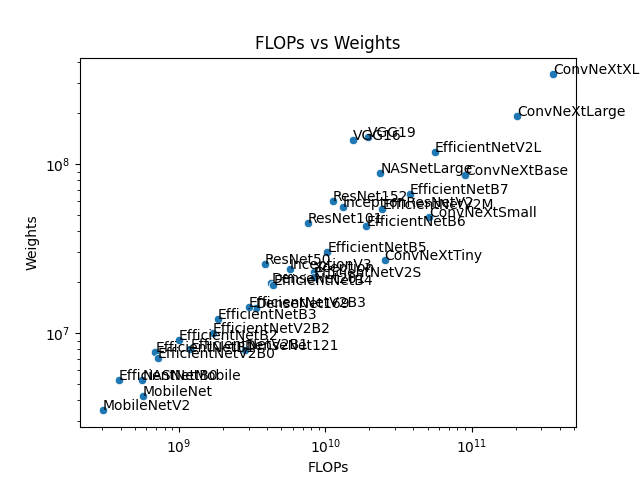
\includegraphics[clip, height=12cm, bb=-60 0 640 480]{data/figure/models_info.png}
		\caption{モデルごとのFLOPsとWeights}
		\label{flops_vs_weights}
	\end{center}
\end{figure}


計算機の資源,特にGPUやスーパーコンピュータの性能も向上しているが,スマートフォンやスマートカメラなど計算資源が限られているエッジデバイスでは,実行可能なモデルも制限される.

% --- T.B.D ---
市場規模

業界団体
	TinyML

企業

